\newpage
\chapter{Projektmanagement}
\section{Vorgehensmodell}
Das Vorgehensmodell teilt die 15 Wochen der Bachelor Arbeit in drei Blöcke ein. Es sind dies:
\begin{itemize}
\item Recherche \& Theorie Phase
\item Simulation \& Design Phase
\item Funktionsmuster \& Verifikation Phase
\end{itemize}
Die zur Verfügung stehende Zeit wird allen drei Blöcken zu gleichen Teilen zugeteilt. In der Abbildung \ref{Vorgehensmodell} sind die drei Projektblöcke gezeigt. Jeder Block endet mit einem Meilenstein und die Zwischenpräsentation stellt ebenfallse einen eigenen Meilenstein dar. 
\begin{figure}[!ht]
	\begin{center}
		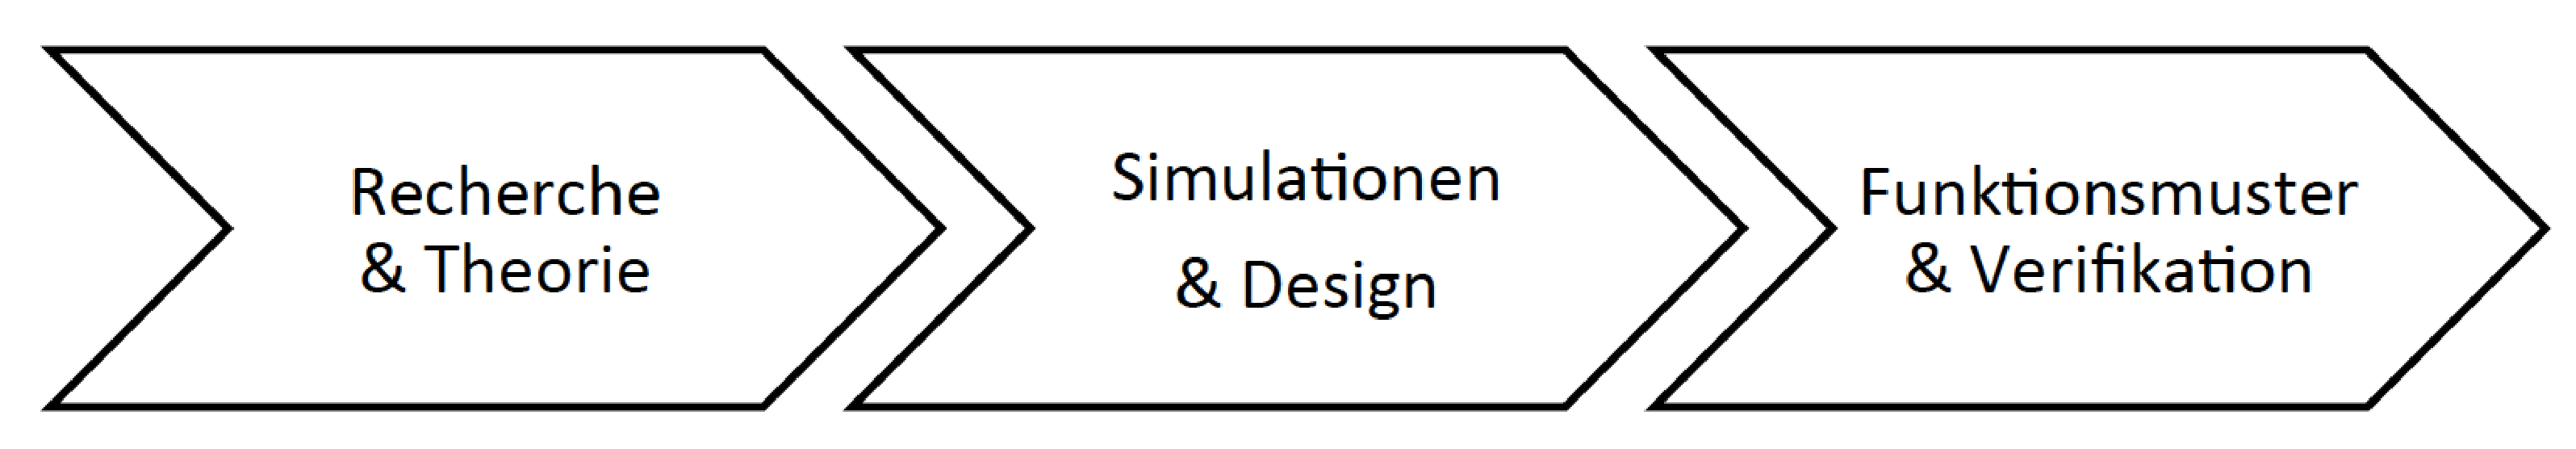
\includegraphics[width=16cm]{content/bilder/Vorgehensmodell.pdf}%
	\end{center}
	\caption{Vorgehensmodell}
	\label{Vorgehensmodell}
\end{figure}
\section{Meilensteine}
Anhand der Blöcke des Vorgehensmodells werden die folgenden vier Meilensteine definiert. Die Meilensteine markieren jeweils das Ende einer Projektphase und haben einen Fertigstellungstermin. Beim Erreichen eines Meilensteins wird die bisherige Arbeit bewertet und Beschlüsse über den weiteren Projektverlauf gefällt. Insgesamt dienen die Meilensteine dem Projektcontrolling.
%\todo{fünf Meilensteine definieren}
	\begin{itemize}
		\item MS1: Theorie und Recherchephase abgeschlossen und zu 80\% dokumentiert, ein Anforderungsdokument wurde erstellt
		\item MS2: Zwischenpräsentation, Vorstellen der ersten vier Antennenkonzepte
		\item MS3: Design und Prototyping, Antennensystem simulieren, produzieren, messen und bewerten
		\item MS4: Engineeringmodel ist gefertigt und dokumentiert
	\end{itemize}




\subsection{Arbeitspakete}
Der Meilenstein 1 schliesst die Recherche und Theorie Phase ab. Die wesentlichen Arbeitspakete sind:
\begin{itemize}
\item Untersuchen, Verstehen und Beschreiben des Abstrahlverhalten von Elementarstrahlern
\item Die elektromagnetische Feldausbreitung soweit  verstehen, um diese in einfachen Worten zu beschreiben.
\item Den Zusammenhang von Richtcharakteristik, Wirkungsgrad und Gewinn von verschieden Antennen verstehen und dokumentieren
\item Untersuchen, Verstehen und Beschreiben der Impedanz von Elementarstrahlern
\end{itemize}
Der Meilenstein 2 beschreibt die Zwischenpräsentation. Dabei wurden die ersten Resultate aus der Theorie,  die ersten Erkenntnisse aus den Simulationen und erste Schlüsse aus dem Vergleich, der idealisierten Theorie und den Simulationen gezogen. 
Konkret wurden die folgenden Punkte gezeigt:
\begin{itemize}
\item Das Vorgehensmodell zeigt die Herangehensweise an die BDA
\item Die Feldausbreitung der Elementarstrahler
\item Die Miniaturisierung von Antennen und deren Auswirkung auf Antennenparameter wie: Strahlungswiderstand, Impedanz, Frequenzverschiebung
\item Anhand des Ersatzschaltbildes von einer Hochfrequenzquelle, Leitungen und von einer Antenne wurden Anpassungsschwierigkeiten besprochen
\end{itemize}
Der 3. Meilenstein beinhaltet verschiedenste Arbeitspakete, um einige zu nennen:
\begin{itemize}
\item Impedanz und Resonanzfrequenz  bei Verkürzung von Antennen simulieren
\item die Richtcharakteristik von Loop- und Dipolantennen analysieren und Vor- und Nachteile für die Antennen bewerten
\item Konkrete, umsetzbare Antennendesigns für den Einsatz im Fluggerät finden, simulieren und bewerten
\end{itemize}
Der Meilenstein drei endet mit einem konkreten Design welches hergestellt, ausgemessen und bewertet wird.\\
Der 4. Meilenstein beinhaltet das Ausmessen und Bewerten des Funktionsmusters.
\begin{itemize}
\item Funktionsmuster aus den Designs erstellen
\item Messen der Antennenparameter
\item Vergleich der Simulationen mit den Messwerten
\item Interpretation des Antennendesign und Vergleich mit den Anforderung 
\item Beurteilung des Antenne für den weitern Einsatz in den Fluginstrumenten der Flytec AG. 
\end{itemize}

\subsection{Ressourcenplanung}
Für die Bachelor Diplom Arbeit wird eine Zeitraum von ca. 360 Stunden eigeplahnt. Diese Zeit wird auf 15 Wochen mit je drei Arbeitstagen verteilt. Für die drei Arbeitsphasen wurden je etwa dieselbe Zeit, das bedeutet je 5 Wochen, eigeplant.\\
Da ausser dem Betreuer Prof. Marcel Joss, dem Industripartner vertreten durch Erich Lerch  und dem Experten Hanspeter Oppliger keine weiteren Personen in die Arbeit involviert sind, können die Arbeitspakete individuell bearbeitet werden und es muss nicht auf Drittpersonen Rücksicht genommen werden.\\
Die Messeinrichtung wurde während der 3. Arbeitsphase der "Funktionsmuster und Verifikation" $\ $nur noch vom Wissenschaftlichen Mitarbeiter und Masterstudent Tobias Plüss verwendet. Es musste, keinerlei Planung stattfinden, um  Überschneidungen der Mess- und Analysezeiten zutreffen zu umgehen. 

\subsection{Risikoanalyse}
Wie in der Resourcenplanung erwähnt, war es nicht nötig mit externen Stellen und Drittpersonen für die Erreichung der Ziele der Bachelor Diplom Arbeit zusammen zu arbeiten. Das heisst es besteht keinerlei Risiko aufgrund der Zusammenarbeit mit externe Stellen.\\
Weiter werden keine Printantennen in Auftragt gegeben die lange Wartezeiten mit sich bringen.
Die Messeinrichtung stellt auch kein Risiko dar, denn von den meisten Messgeräten sind mehrere oder vergleichbare Exemplare vorhanden.\\
Eine Ausnahme stellt das StarLab dar. Von dieses Antennenmessgerät ist nur eines an der Hochschule für Technik und Architektur vorhanden. Daher muss auf die einwandfreie Funktion diese vertraut werden. Ist das Gerät nicht funktionstüchtig können keine Abstrahlcharakteristiken des Funktionsmuster aufgenommen werden.

\section{Projektsitzungen und Gesprächsnotizen}
Die Gesprächsnotizen dienen dazu den  Projektverlauf nachvollziehbar zu dokumentieren. Sie werden jeweils nach den Projektsitzungen mit dem Betreuer Prof. Marcel Joss für die kommende Woche erstellt. Die jeweiligen Arbeitspakete von der vergangenen Woche und der kommenden Woche werden an den Sitzungen besprochen und dokumentiert. Beschlüsse, die für den Verlauf der BDA relevant sind, werden besprochen und dokumentiert.



